\section{Secondary input parameters 辅助输入参数}

\begin{paracol}{2}

    A possible reason for the significant data scatter around the mean trend is that additional explanatory variables are not incorporated into the transformation model. As a result, the variation in these hidden explanatory variables, which is inevitable in a database, is added to the transformation uncertainty. A good example is the $\rm{OCR}-(s_u/\sigma_v')$ model by \citet{Jamiolkowski198557}. The COV with respect to the global database is 0.53 for this model (see \autoref{table:5}). This means that the standard deviation of the data scatter is about 53$\%$ of the mean trend. A possible hidden explanatory variable is the sensitivity $S_t$ — it is known that the “stress history and normalized soil engineering properties” SHANSEP parameters for sensitive (structured) clays are different from those for insensitive clays. In fact, by incorporating $S_t$ as a secondary input parameter, the $\rm{OCR}-(s_u/\sigma_v')-S_t$ model by \cite{Ching2012522}carries a significantly smaller COV of 0.34 (see \autoref{table:5}). It is widely known that parameters such as PI and $S_t$ can be applied as secondary explanatory variables for some correlations. It is of interest to see whether the incorporation of these secondary input parameters can reduce COV significantly. If the COV reduction is significant, it is of interest to re-calibrate the transformation models to further update the bias factors and the COVs in \autoref{table:5}. This is the main objective of this section.

    \switchcolumn

    围绕平均趋势出现大量数据分散的可能原因是,其他解释变量未合并到转换模型中。结果,这些隐藏的解释变量的变化(这在数据库中是不可避免的)被添加到变换不确定性中。一个很好的例子是\citet{Jamiolkowski198557}的$\rm{OCR}-(s_u/\sigma_v')$模型。对于此模型,相对于全局数据库的COV为0.53(请参见\cntableref{table:5})。这意味着数据散布的标准偏差约为平均趋势的53$\%$。可能的隐藏解释变量是敏感度$S_t$ - 已知敏感(结构化)黏土的“应力历史和规范化的土体工程特性” SHANSEP参数与不敏感黏土的参数不同。实际上,通过将$S_t$作为次要输入参数,\cite{Ching2012522}的$\rm{OCR}-(s_u/\sigma_v')-S_t$模型携带的COV值要小得多,为0.34(参见\cntableref{table:5})。众所周知,诸如PI和$S_t$之类的参数可以用作某些相关性的次要解释变量。有趣的是,这些辅助输入参数的合并是否可以显着降低COV。如果COV降低很大,则需要重新校准转换模型以进一步更新\cntableref{table:5}中的偏置因子和COV。这是本节的主要目标。

    \switchcolumn*[\Paragraph{Correlation between $\epsilon$ and $(\rm{PI}, S_t)$ $\epsilon$与$(\rm{PI}, S_t)$之间的相关性}]

    Let us recall from \autoref{equation:1} that the variability term $\epsilon$ for a  transformation model can be expressed as

    \switchcolumn

    让我们从\cnequationref{equation:1}中回忆,转换模型的可变性项$\epsilon$可以表示为
\end{paracol}

\begin{align}
    \epsilon=\dfrac{\rm{actual~target~value}}{b\times{}\rm{predicted~target~value}}=\dfrac{\rm{actual~target~value}}{\rm{unbiased~prediction}}
    \label{equation:2}
\end{align}

\begin{paracol}{2}

    where the unbiased prediction = $b\times$ predicted target value. The variability term epsilou quantifies the deviation between the actual value and the unbiased prediction. It has mean value of 1 and COV equation to the calibrated COV (delta). Equivalently

    \switchcolumn

    其中无偏预测 = $b\times$预测目标值。 可变性项$\varepsilon$量化了实际值和无偏预测之间的偏差。它的平均值为1,且COV等于校准的COV($\delta$)。等效地,
\end{paracol}

\begin{align}
    \ln(\varepsilon)=\ln(\rm{actual~target~value})-\ln({\rm{unbiased~prediction}})
    \label{equation:3}
\end{align}

\begin{paracol}{2}

    In essence, $\ln(\varepsilon)$ is the component that cannot be explained away by the primary input parameter. More precisely, $\ln(\varepsilon)$ should be uncorrelated to the primary input parameter. The reason why the natural logarithm is taken will be explained later. For instance, $\ln(\varepsilon)$ for the $\rm{OCR}-(s_u/\sigma_v')$ model proposed by \citet{Jamiolkowski198557} is indeed nearly uncorrelated to the primary input parameter $\ln(\rm{OCR})$, shown in \autoref{figure:16}a. Incidentally, the correlation between $\ln(\varepsilon)$ and $\ln(\rm{PI})$ is also nearly zero (\autoref{figure:16}b). However, $\ln(\varepsilon)$ and $\ln(S_t)$ show some slight positive correlation (\autoref{figure:16}c). In this case, it may be possible to adopt St as the secondary input parameter for Jamiolkowski et al.’s model to reduce its COV.

    \switchcolumn

    本质上,$\ln(\varepsilon)$是无法由主输入参数解释的成分。 更准确地说,$\ln(\varepsilon)$应该与主要输入参数不相关。 取自然对数的原因将在后面说明。 例如,\citet{Jamiolkowski198557}提出的$\rm{OCR}-(s_u/\sigma_v')$模型的$\ln(\varepsilon)$的确与\cnfigureref{figure:16}a所示的主要输入参数$\ln(\rm{OCR})$几乎不相关。 顺便提及,$\ln(\varepsilon)$和$\ln(\rm{PI})$之间的相关性也几乎为零(\cnfigureref{figure:16}b)。 但是,$\ln(\varepsilon)$和$\ln(S_t)$表现出一些轻微的正相关(\cnfigureref{figure:16}c)。 在这种情况下,有可能采用$S_t$作为Jamiolkowski等人模型的辅助输入参数,以降低其COV。

    \begin{figure}[!htb]
    \centering
    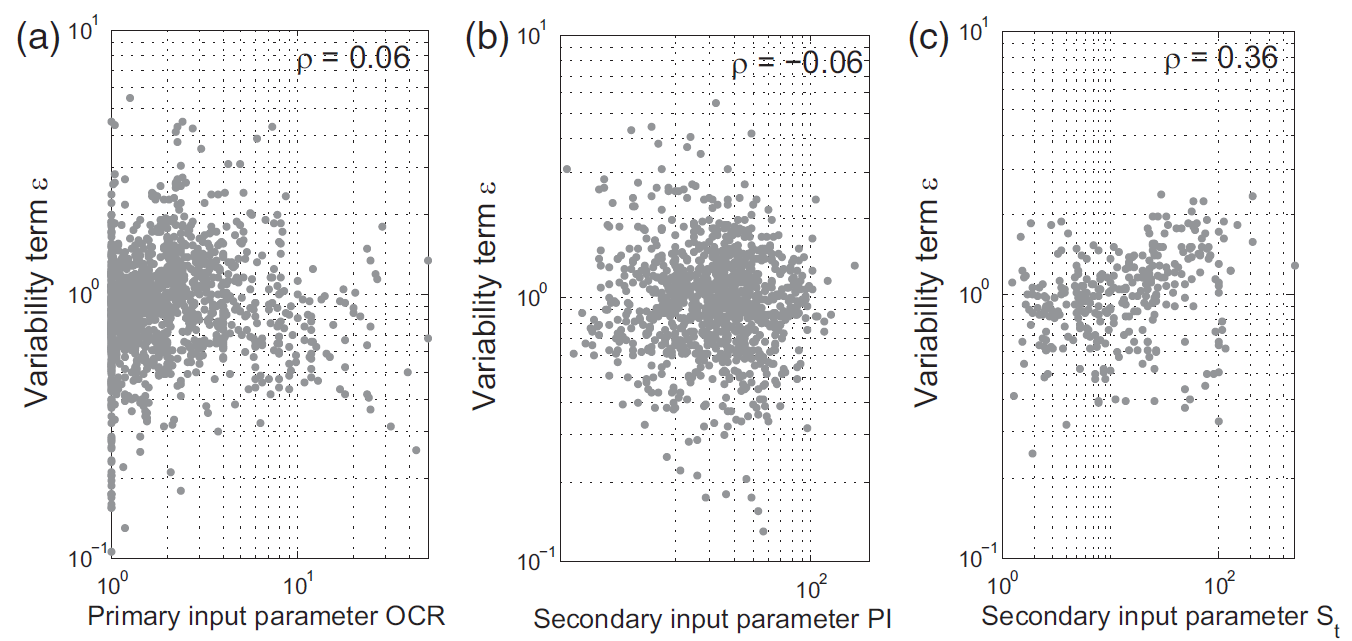
\includegraphics[width=0.7\textwidth]{figures/figure-16.png}
    \caption{(a) $\ln(\varepsilon)–\ln(\rm{OCR})$, (b) $\ln(\varepsilon)–\ln(\rm{PI})$, and (c) $\ln(\varepsilon)–\ln(S_t)$ plots for the model proposed by \citet{Jamiolkowski198557}. $\rho$, correlation coefficient.}
    \addtocounter{figure}{-1}
    \vspace{-5pt}
    \renewcommand{\figurename}{图}
    \caption{(a) $\ln(\varepsilon)–\ln(\rm{OCR})$, (b) $\ln(\varepsilon)–\ln(\rm{PI})$, and (c) $\ln(\varepsilon)–\ln(S_t)$ \citet{Jamiolkowski198557}提出的模型的图解。 $\rho$,相关系数。}
    \renewcommand{\figurename}{Figure}
    \label{figure:16}
\end{figure}
    \switchcolumn*

    In this section, the correlation between $\ln(\epsilon)$ and the natural logarithm of the secondary input parameter (PI or $S_t$) will be  studied. The correlation with respect to $\ln(\rm{PI})$ will be studied for all models except the $\rm{PI}-(s_u/\sigma_p')$ model proposed by \citet{Mesri1975409, Mesri1989162}, because PI is already the primary input parameter. Similarly, the correlation with respect to $\ln(S_t)$ will not be studied for models whose primary inputs already involve $S_t$. The correlation with respect to $\ln(S_t)$ will not be studied for models whose target is $s_u^{re}$, because soil structure is supposed to be destroyed in the  remoulded state and hence, it does not make much sense to infer $s_u^{re}$ using $S_t$.

    \switchcolumn

    在本节中,将研究$\ln(\epsilon)$与辅助输入参数(PI或$S_t$)的自然对数之间的相关性。 因为PI已经是主要的输入参数,所以将研究除\citet{Mesri1975409, Mesri1989162}提出的$\rm{PI}-(s_u/\sigma_p')$模型以外的所有模型与$\ln(\rm{PI})$的相关性。 同样,对于主要输入已经包含$S_t$的模型,将不会研究与$\ln(S_t)$的相关性。对于目标为$s_u^{re}$的模型,将不会研究与$\ln(S_t)$的相关性,因为应该在重塑状态下破坏土体结构,因此使用$S_t$推断$s_u^{re}$没有太大意义。

    \switchcolumn*

    The correlation between $\ln(\epsilon)$ and the natural logarithm of the secondary input parameter (PI or $S_t$) is quantified by the Pearson product moment correlation coefficient ($\rho$). The correlation coefficient for the $\ln(\epsilon)-\ln(\rm{PI})$ and $\ln(\epsilon)-\ln(S_t)$ correlations are shown in Table 6. The parameter n shown in Table 6 is the number of data points used to estimate each correlation. It is clear that the $\ln(\epsilon)-\ln(\rm{PI})$ data points are abundant ($n$ > 300), whereas the $\ln(\epsilon)-\ln(S_t)$ data points are less abundant. It is also evident that the $\ln(\epsilon)-\ln(S_t)$ correlations seem stronger ($\rho$ is farther away from zero) than the $\ln(\epsilon)-\ln(\rm{PI})$ correlations.

    \switchcolumn

    $\ln(\epsilon)$和辅助输入参数(PI或$S_t$)的自然对数之间的相关性通过皮尔逊乘积矩相关系数($\rho$)进行量化。 $\ln(\epsilon)-\ln(\rm{PI})$和 $\ln(\epsilon)-\ln(S_t)$相关性的相关系数如\cntableref{table:6}所示。\cntableref{table:6}中所示的参数$n$是用于估计每个相关性的数据点数。 显然,$\ln(\epsilon)-\ln(\rm{PI})$数据点数量丰富($n$ > 300),而$\ln(\epsilon)-\ln(S_t)$数据点数量较少。 同样明显的是,$\ln(\epsilon)-\ln(S_t)$相关性似乎比$\ln(\epsilon)-\ln(\rm{PI})$相关性更强($\rho$离零更远)。
\end{paracol}

\newcommand{\RelationshipA}{$\rm{LI}-s_u^{re}/P_a$}
\newcommand{\RelationshipB}{$\rm{LI}-S_t$}
\newcommand{\RelationshipC}{$\rm{LI}-\sigma_p'/P_a-S_t$}
\newcommand{\RelationshipD}{$\rm{PI}-s_u/\sigma_p'$}
\newcommand{\RelationshipE}{$\rm{OCR}-s_u/\sigma_p'$}
\newcommand{\RelationshipF}{$\rm{OCR}-s_u/\sigma_p'-S_t$}
\newcommand{\RelationshipG}{$\rm{CPTU}-s_u/\sigma_p'$}
\newcommand{\RelationshipH}{$\rm{CPTU}-\rm{OCR}$}
\newcommand{\RelationshipI}{$\rm{CPTU}-\sigma_p'/P_a$}

\newcommand{\LiteratureA}{\citet{Locat1988799}}
\newcommand{\LiteratureB}{\citet{Bjerrum195449}}
\newcommand{\LiteratureC}{\citet{Ching2012522}}
\newcommand{\LiteratureD}{\citet{Stas1984}}
\newcommand{\LiteratureE}{\citet{Ching2012522}}
\newcommand{\LiteratureF}{\citet{Mesri1975409,Mesri1989162}}
\newcommand{\LiteratureG}{\citet{Jamiolkowski198557}}
\newcommand{\LiteratureH}{\citet{Ching2012522}}
\newcommand{\LiteratureI}{\citet{Ching201252}}
\newcommand{\LiteratureJ}{\citet{Chen1996488}}
\newcommand{\LiteratureK}{\citet{Kulhawy1990}}
\newcommand{\LiteratureL}{\citet{Chen1996488}}
\newcommand{\LiteratureM}{\citet{Kulhawy1990}}

\newcommand{\UModelA}{$s_u^{re}/P_a\approx{}0.0144\rm{LI}^{-2.44}b'\varepsilon'$}
\newcommand{\UModelB}{$S_t\approx10^{0.8\rm{LI}}b'\varepsilon'$}
\newcommand{\UModelC}{$S_t\approx{}20.726\rm{LI}^{1.910}b'\varepsilon'$}
\newcommand{\UModelD}{\makecell[l]{$\sigma_p'/P_a\approx{}10^{1.11-1.62\rm{LI}}b'\varepsilon'$\\(for $S_t < 10$ only)}}
\newcommand{\UModelE}{$\sigma_p'/P_a\approx{}0.235\rm{LI}^{-1.319}S_t^{0.536}b'\varepsilon'$}
\newcommand{\UModelF}{$s_u(\rm{mob})/\sigma_p'\approx{}0.22b'\varepsilon'$}
\newcommand{\UModelG}{$s_u(\rm{mob})/\sigma_p'\approx{}0.23(\rm{OCR})^{0.8}b'\varepsilon'$}
\newcommand{\UModelH}{$s_u(\rm{mob})/\sigma_p'\approx{}0.229(\rm{OCR})^{0.823}S_t^{0.121}b'\varepsilon'$}
\newcommand{\UModelI}{$\dfrac{\left[(q_t-\sigma_v)/\sigma_v'\right]}{\left[s_u(\rm{mob})/\sigma_v'\right]}\approx{}29.1\exp(-0.513B_q)b'\varepsilon'$}
\newcommand{\UModelJ}{$\dfrac{\left[(q_t-u_2)/\sigma_v'\right]}{\left[s_u(\rm{mob})/\sigma_v'\right]}\approx{}34.6\exp(-2.049B_1)b'\varepsilon'$}
\newcommand{\UModelK}{$\dfrac{\left[(u_2-u_0)/\sigma_v'\right]}{\left[s_u(\rm{mob})/\sigma_v'\right]}\approx{}21.5B_qb'\varepsilon'$}
\newcommand{\UModelL}{$\rm{OCR}\approx{}0.259\left[(q_t-\sigma_v')\right]^{1.107}b'\varepsilon'$}
\newcommand{\UModelM}{$\rm{OCR}\approx{}0.545\left[(q_t-u_2)\right]^{0.969}b'\varepsilon'$}
\newcommand{\UModelN}{$\rm{OCR}\approx{}1.026B_q^{-1.077}b'\varepsilon'$}
\newcommand{\UModelO}{$\rm{OCR}\approx{}0.32\left[(q_t-\sigma_v)/\sigma_v'\right]b'\varepsilon'$}
\newcommand{\UModelP}{$\sigma_p'/P_a\approx{}0.227\left[(q_t-\sigma_v)/P_a\right]^{1.200}b'\varepsilon'$}
\newcommand{\UModelQ}{$\sigma_p'/P_a\approx{}0.490\left[(q_t-u_2)/P_a\right]^{1.053}b'\varepsilon'$}
\newcommand{\UModelR}{$\sigma_p'/P_a\approx{}\left[1.274+0.761(u_2-u_0)/P_a\right]b'\varepsilon'$}
\newcommand{\UModelS}{$\sigma_p'/P_a\approx{}0.33\left[(q_t-\sigma_v)/P_a\right]b'\varepsilon'$}
\newcommand{\UModelT}{$\sigma_p'/P_a\approx{}0.54\left[(u_2-u_0)/P_a\right]b'\varepsilon'$}

    \begin{sidewaystable}[!p]
        \centering
        \scriptsize
        \renewcommand\arraystretch{1.7}
        \caption{Analysis results for $\ln(\varepsilon)-\ln(\rm{PI})$ and $\ln(\varepsilon)-\ln(S_t)$ correlations and inference results.}
        \addtocounter{table}{-1}
        \vspace{-8pt}
        \renewcommand{\tablename}{表}
        \caption{$\ln(\varepsilon)-\ln(\rm{PI})$和$\ln(\varepsilon)-\ln(S_t)$相关性和推断分析结果。}
        \vspace{4pt}
        \renewcommand{\tablename}{Table}
        \setlength{\tabcolsep}{0.4mm}{
        \begin{tabular}{lllllllllll}
            \toprule
                            &               & \multicolumn{4}{l}{\footnotesize Correlation coefficient}      &       & \multicolumn{4}{l}{\footnotesize Inference results} \\
                            &               & \multicolumn{2}{l}{\footnotesize $\varepsilon-$PI} & \multicolumn{2}{l}{\footnotesize $\varepsilon-S_t$}  &       & \multicolumn{2}{l}{\footnotesize Inference based PI only} & \multicolumn{2}{l}{\footnotesize Inference based on PI and $S_t$} \\
                            \footnotesize{Relationship}   & \footnotesize{Literature}    &  \footnotesize{$n$} &  \footnotesize{$\rho$} &  \footnotesize{$n$} & \footnotesize{$\rho$} &  \footnotesize{Updated model} &  \footnotesize{$b'=b\times{}[\rm{BCF}]$} &  \footnotesize\makecell{$\delta'=$\\$\delta\times{}[\rm{CCF}\%]$} &  \footnotesize{$b'=b\times{}[\rm{BCF}]$} & \footnotesize\makecell{$\delta'=$\\$\delta\times{}[\rm{CCF}\%]$} \\
            \midrule
            \RelationshipA  & \LiteratureA & 887  & -0.24 & $-$   & $-$     & \UModelA & $1.92\times{}\left[1.11(\rm{PI}/20)^{-0.258}\right]$ & $1.25\times{}( 94\%)$ & $-$ & $-$ \\
            \RelationshipB  & \LiteratureB & 1137 & 0.18  & $-$   & $-$     & \UModelB & $2.05\times{}\left[0.92(\rm{PI}/20)^{ 0.251}\right]$ & $1.09\times{}(104\%)$ & $-$ & $-$ \\
                            & \LiteratureC & 1137 & -0.02 & $-$   & $-$     & \UModelC & $0.88\times{}\left[0.88(\rm{PI}/20)^{-0.025}\right]$ & $1.28\times{}( 99\%)$ & $-$ & $-$ \\
            \RelationshipC  & \LiteratureD & 257  & -0.37 & $-$   & $-$     & \UModelD & $2.94\times{}\left[2.94(\rm{PI}/20)^{-0.478}\right]$ & $1.90\times{}( 85\%)$ & $-$ & $-$ \\
                            & \LiteratureE & 487  & -0.35 & $-$   & $-$     & \UModelE & $1.32\times{}\left[1.32(\rm{PI}/20)^{-0.444}\right]$ & $0.78\times{}( 78\%)$ & $-$ & $-$ \\
            \RelationshipD  & \LiteratureF & $-$    & $-$     & 433 & 0.43  & \UModelF &                                                      &                       & $1.04\times{}\left[0.76S_t^{0.136}\right]$ & $0.55\times{}(63\%)$ \\
            \RelationshipE  & \LiteratureG & 1091 & -0.06 & 395 & 0.34  & \UModelG & $1.11\times{}\left[1.11(\rm{PI}/20)^{-0.050}\right]$ & $0.53\times{}( 53\%)$ & $1.11\times{}\left[0.71(\rm{PI}/20)^{ 0.133}S_t^{ 0.123}\right]$ & $0.53\times{}(67\%)$ \\
            \RelationshipF  & \LiteratureH & 391  & 0.21  & $-$   & $-$     & \UModelH & $0.84\times{}\left[0.84(\rm{PI}/20)^{ 0.131}\right]$ & $0.34\times{}( 34\%)$ & $-$ & $-$ \\
            \specialrule{0em}{2pt}{2pt}
            \RelationshipG  & \LiteratureI & 387  & 0.38  & 81  & -0.24 & \UModelI & $0.95\times{}\left[0.95(\rm{PI}/20)^{ 0.348}\right]$ & $0.49\times{}( 49\%)$ & $0.95\times{}\left[1.17(\rm{PI}/20)^{ 0.133}S_t^{-0.198}\right]$ & $0.49\times{}(66\%)$ \\
            \specialrule{0em}{2pt}{2pt}
                            &              & 392  & 0.29  & 78  & -0.39 & \UModelJ & $1.11\times{}\left[1.11(\rm{PI}/20)^{ 0.275}\right]$ & $0.57\times{}( 57\%)$ & $1.11\times{}\left[1.40(\rm{PI}/20)^{ 0.241}S_t^{-0.263}\right]$ & $0.57\times{}(72\%)$ \\
            \specialrule{0em}{2pt}{2pt}
                            &              & 387  & 0.38  & 81  & -0.25 & \UModelK & $0.94\times{}\left[0.94(\rm{PI}/20)^{ 0.335}\right]$ & $0.49\times{}( 49\%)$ & $0.94\times{}\left[1.22(\rm{PI}/20)^{ 0.189}S_t^{-0.216}\right]$ & $0.49\times{}(78\%)$ \\
            \specialrule{0em}{2pt}{2pt}
            \RelationshipH  & \LiteratureJ & 497  & -0.09 & 163 & 0.12  & \UModelL & $1.01\times{}\left[1.01(\rm{PI}/20)^{-0.073}\right]$ & $0.42\times{}( 42\%)$ & $1.01\times{}\left[1.09(\rm{PI}/20)^{ 0.275}S_t^{ 0.002}\right]$ & $0.42\times{}(73\%)$ \\
                            &              & 466  & -0.11 & 123 & 0.27  & \UModelM & $1.06\times{}\left[1.06(\rm{PI}/20)^{-0.105}\right]$ & $0.57\times{}( 57\%)$ & $1.06\times{}\left[0.79(\rm{PI}/20)^{-0.206}S_t^{ 0.102}\right]$ & $0.57\times{}(69\%)$ \\
                            &              & 545  & -0.17 & 173 & 0.12  & \UModelN & $1.28\times{}\left[1.28(\rm{PI}/20)^{-0.196}\right]$ & $0.86\times{}( 86\%)$ & $1.28\times{}\left[0.63(\rm{PI}/20)^{-0.079}S_t^{-0.057}\right]$ & $0.86\times{}(52\%)$ \\
                            & \LiteratureK & 497  & -0.11 & 163 & 0.14  & \UModelO & $1.00\times{}\left[1.00(\rm{PI}/20)^{-0.084}\right]$ & $0.39\times{}( 39\%)$ & $1.00\times{}\left[1.04(\rm{PI}/20)^{-0.188}S_t^{ 0.010}\right]$ & $0.39\times{}(71\%)$ \\
            \RelationshipI  & \LiteratureL & 497  & -0.04 & 163 & 0.15  & \UModelP & $0.99\times{}\left[0.99(\rm{PI}/20)^{-0.028}\right]$ & $0.42\times{}( 42\%)$ & $0.99\times{}\left[1.07(\rm{PI}/20)^{-0.124}S_t^{ 0.002}\right]$ & $0.42\times{}(70\%)$ \\
                            &              & 466  & -0.09 & 123 & 0.28  & \UModelQ & $1.08\times{}\left[1.08(\rm{PI}/20)^{-0.087}\right]$ & $0.61\times{}( 61\%)$ & $1.08\times{}\left[0.78(\rm{PI}/20)^{-0.268}S_t^{ 0.205}\right]$ & $0.61\times{}(68\%)$ \\
                            &              & 498  & -0.25 & 163 & 0.04  & \UModelR & $0.49\times{}\left[0.49(\rm{PI}/20)^{-0.235}\right]$ & $0.59\times{}( 59\%)$ & $1.49\times{}\left[0.94(\rm{PI}/20)^{-0.262}S_t^{ 0.026}\right]$ & $0.59\times{}(60\%)$ \\
                            & \LiteratureM & 497  & -0.11 & 163 & 0.14  & \UModelS & $0.97\times{}\left[0.97(\rm{PI}/20)^{-0.084}\right]$ & $0.39\times{}( 39\%)$ & $0.97\times{}\left[1.04(\rm{PI}/20)^{-0.188}S_t^{ 0.010}\right]$ & $0.39\times{}(71\%)$ \\
                            &              & 497  & -0.12 & 162 & -0.01 & \UModelT & $1.18\times{}\left[1.18(\rm{PI}/20)^{-0.114}\right]$ & $0.75\times{}( 75\%)$ & $1.18\times{}\left[1.04(\rm{PI}/20)^{-0.114}S_t^{-0.069}\right]$ & $0.75\times{}(61\%)$ \\
            \bottomrule
        \end{tabular}}%
        \label{table:6}%
        \renewcommand\arraystretch{1.0}
    \end{sidewaystable}

\begin{paracol}{2}
    \switchcolumn[0]*[\Paragraph{Re-calibrate the existing transformation models - inference using PI and $S_t$ 重新校准现有的转换模型-使用PI和$S_t$进行推断}]

    For the inference using PI, it is possible to express $\varepsilon$ as a function of PI

    \switchcolumn

    对于使用PI进行推理,可以将$\varepsilon$表示为PI的函数
\end{paracol}

\begin{align}
    \varepsilon=\left[\alpha(\rm{PI}/20)^\beta\right]\varepsilon'
    \label{equation:4}
\end{align}

\begin{paracol}{2}
     where $\varepsilon'$ is the (updated) variability term that cannot be explained away by PI, and PI = 20 is a reference PI value (median plasticity). The mean value of $\varepsilon'$ is still 1 and its (updated) COV is denoted by $\delta'$, which should be less than $\delta$ if $\ln(\varepsilon)$ and $\ln(\rm{PI})$ are correlated. The coefficients $\alpha$ and $\beta$ can be estimated using linear regression on the $\ln(\varepsilon)-\ln(\rm{PI})$ data points. Namely, the following regression model is used:

    \switchcolumn

    其中$\varepsilon'$是无法由PI解释的(更新的)可变性项,而PI = 20是一个参考PI值(中位数可塑性)。 $\varepsilon'$的平均值仍为1,并且其(更新的)COV用$\delta'$表示,如果$\ln(\varepsilon)$和$\ln(\rm{PI})$相关,则其应小于$\delta$。 可以使用$\ln(\varepsilon)-\ln(\rm{PI})$数据点上的线性回归来估计系数$\alpha$和$\beta$。 即,使用以下回归模型:

\end{paracol}

\begin{align}
    \ln(\varepsilon)\approx{}\ln(\alpha)+\beta\ln(\rm{PI}/20)
    \label{equation:5}
\end{align}

\begin{paracol}{2}
    where $\ln(\varepsilon)$ is the known output and $\ln(\rm{PI}/20)$ is the known input, whereas $\ln(\alpha)$ and $\beta$ are the intersect and gradient, respectively, to be estimated by the least squares method. The natural logarithm is taken for $varepsilon$ and PI because traditional linear regression requires normality. \autoref{figure:17} shows the histograms of $\varepsilon$ and $\ln(\varepsilon)$ for the $\rm{OCR}-(s_u/\sigma_v')$ model proposed by \citet{Jamiolkowski198557} - $\ln(\varepsilon)$ is more normal than $\varepsilon$. In fact, $\ln(\rm{PI})$ is also more normal than PI (not shown). Hence, it is more appropriate to do regression on the $\ln(\varepsilon)-\ln(\rm{PI})$ data points. Once the least-squares estimates for $\alpha$ and $\beta$ are obtained, \autoref{equation:1} can be expressed as

    \switchcolumn

    其中$\ln(\varepsilon)$是已知输出,而$\ln(\rm{PI}/20)$是已知输入,而$\ln(\alpha)$和$\beta$是分别通过最小二乘法估计的相交和渐变。 因为传统的线性回归需要正态性,所以PI取自然对数。 \cnfigureref{figure:17}显示了\citet{Jamiolkowski198557}提出的$\rm{OCR}-(s_u/\sigma_v')$模型的$\varepsilon$和$\ln(\varepsilon)$的直方图 - $\ln(\varepsilon)$比$\varepsilon$更为正常。 实际上,$\ln(\rm{PI})$也比PI更正常(未显示)。 因此,对$\ln(\varepsilon)-\ln(\rm{PI})$数据点进行回归更合适。 使用最小二乘估计获得$\alpha$和$\beta$,\cnequationref{equation:1}可以表示为

    \begin{figure*}[!htb]
    \centering
    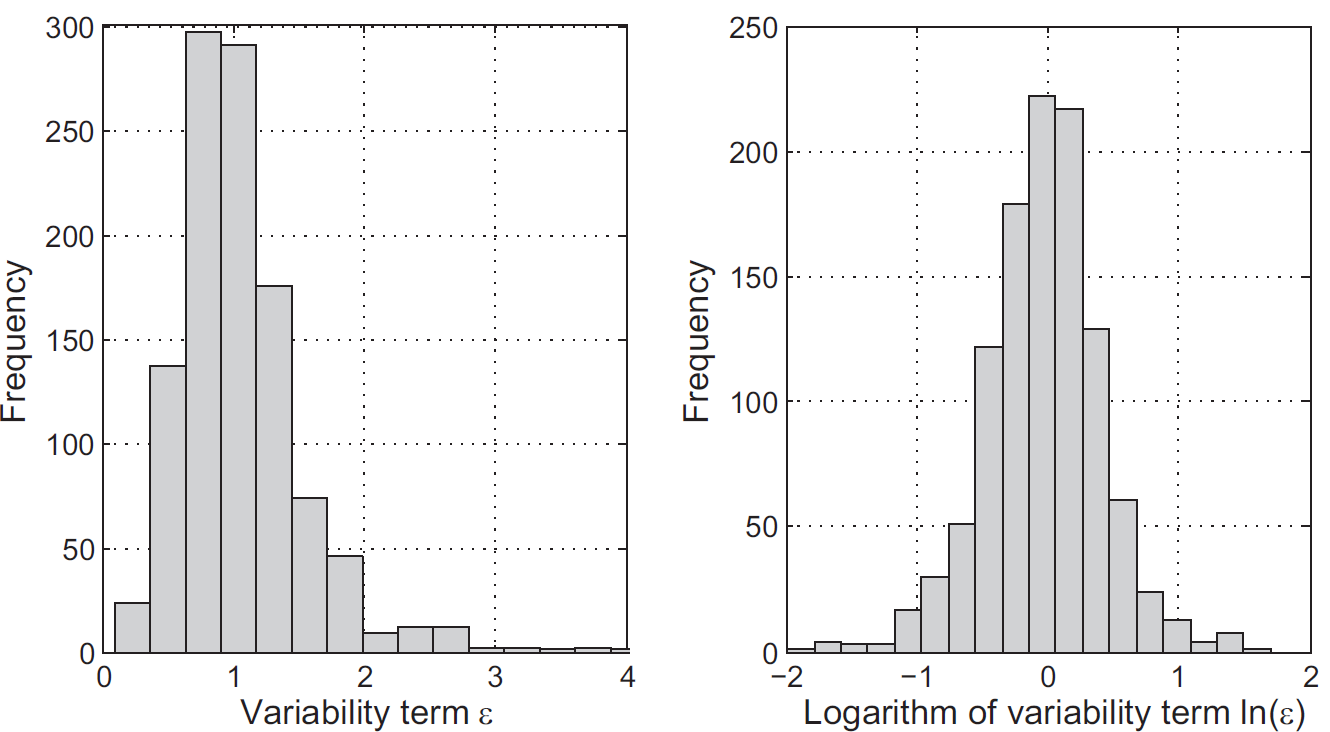
\includegraphics[width=0.5\textwidth]{figures/figure-17.png}
    \caption{Histograms of $\varepsilon$ and $\ln(\varepsilon)$ for the $\rm{OCR}-(s_u/\sigma_v')$ model proposed by \citet{Jamiolkowski198557}.}
    \addtocounter{figure}{-1}
    \vspace{-5pt}
    \renewcommand{\figurename}{图}
    \caption{\citet{Jamiolkowski198557}提出的$\rm{OCR}-(s_u/\sigma_v')$模型的$\varepsilon$和$\ln(\varepsilon)$直方图。}
    \renewcommand{\figurename}{Figure}
    \label{figure:17}
\end{figure*}
\end{paracol}

\begin{align}
        \begin{split}
        \rm{Actual~value}&=\rm{predicted~value}\times{}b\times{}\left[\alpha\times{}(\rm{PI}/20)^\beta\right]\times{}\varepsilon'\\
        &=\rm{predicted~value}\times{}b'\times{}\varepsilon'
    \end{split}
    \label{equation:6}
\end{align}

\begin{paracol}{2}

    where $b'$ is the updated bias factor and can be expressed as the product of the original bias $b$ and a correction term $\alpha\times{}(\rm{PI}/20)^\beta$

    \switchcolumn

    其中$b'$是更新的偏差因子,可以表示为原始偏差$b$与校正项$\alpha\times{}(\rm{PI}/20)^\beta$的乘积
\end{paracol}

\begin{align}
    b'=b\times{}\left[\alpha\times{}(\rm{PI}/20)^\beta\right]=b\times{}(\rm{bias~correction~factor})
    \label{equation:7}
\end{align}
    
\begin{paracol}{2}

    The term  $\alpha\times{}(\rm{PI}/20)^\beta$ is called the bias correction factor (BCF). In \autoref{table:6}, the updated bias factors $b'$ are shown in the format of $b'=(\rm{original}~b)\times{}[BCF]$. The sample COV of epsilou (the updated variability term) is denoted by delta. In \autoref{table:6}, $\delta'$ values are shown in the format of are shown in the format of $\delta'=(\rm{original}~\delta)\times{}(\rm{CCF}\%)$, where CCF denotes the COV correction factor.

    \switchcolumn

    项$\alpha\times{}(\rm{PI}/20)^\beta$称为偏差校正因子(BCF)。在\cntableref{table:6}中,更新的偏差因子$b'$以$b'=(\rm{original}~b)\times{}[BCF]$的格式显示。 $\varepsilon'$的样本COV(更新的可变性项)$\delta'$。 在\cntableref{table:6}中,$\delta'$以$\delta'=(\rm{original}~\delta)\times{}(\rm{CCF}\%)$的格式显示,其中CCF表示COV校正因子。

    \switchcolumn*

    It is apparent that when the target parameter is $\sigma_p'/P_a$ or OCR, the BCFs are always decreasing functions of PI ($\beta<0$). This implies that clays with larger PI values tend to have lower $\sigma_p'/P_a$ and OCR values. For the $\rm{CPTU}-(s_u/\sigma_v')$ model proposed by \citet{Ching201252}, the target parameter is the CPTU cone factors (namely $(q_t-\sigma_v)/s_u$, $(q_t-u_2)/s_u$ and $(u_2-u_0)/s_u$), the BCFs are increasing functions of PI ($\beta>0$). This implies that clays with larger PI tend to have larger cone factors, hence smaller $s_u$. This observation is known (\citealt{Aas19861,Marsland1988209,Powell1988903}) although it has not been established with statistical rigor using such a large database. The CCFs are fairly close to 100$\%$, indicating that the inference using PI does not significantly reduce the transformation uncertainties.

    \switchcolumn

    显然,当目标参数为$\sigma_p'/P_a$或OCR时,BCF始终是PI的递减函数($\beta<0$)。这意味着具有较大PI值的黏土往往具有较低的$\sigma_p'/P_a$和OCR值。 对于\citet{Ching201252}提出的$\rm{CPTU}-(s_u/\sigma_v')$模型,目标参数是CPTU锥因子(即$(q_t-\sigma_v)/s_u$,$(q_t-u_2)/s_u$,以及$(u_2-u_0)/s_u$),BCF是PI的增函数($\beta>0$)。 这意味着具有较大PI的黏土往往具有较大的圆锥系数,因此$s_u$较小。 这种结论是可信的(\citealt{Aas19861,Marsland1988209,Powell1988903}),尽管还没有使用如此庞大的数据库以统计上的严格性来建立它。 CCF相当接近100$\%$,这表明使用PI进行推理并不能显着减少变换的不确定性。

    \switchcolumn*

    For the inference using PI and $S_t$, it is possible to express $\varepsilon$ as

    \switchcolumn

    对于使用PI和$S_t$进行推理,可以将$\varepsilon$表示为

\end{paracol}

    
\begin{align}
    \varepsilon=\left[\alpha\times{}(\rm{PI}/20)^\beta\times{}S_t^\gamma\right]\times{}\varepsilon'
    \label{equation:8}
\end{align}

\begin{paracol}{2}

        The coefficients  $\alpha$,$\beta$ and $\gamma$ can be estimated using linear regression on the $\ln(\varepsilon)-\ln(\rm{PI})-\ln(S_t)$ data points. Namely, the following regression model is used:

    \switchcolumn

    可以使用$\ln(\varepsilon)-\ln(\rm{PI})-\ln(S_t)$数据点上的线性回归来估计系数$\alpha$,$\beta$和$\gamma$。 即使用以下回归模型:

\end{paracol}

\begin{align}
    \ln(\varepsilon)\approx{}\ln(\alpha)+\beta\ln(\rm{PI}/20)+\gamma\ln(S_t)
    \label{equation:9}
\end{align}

\begin{paracol}{2}

    where $\ln(\varepsilon)$ is the known output, and $\ln(\rm{PI}/20)$ and $\ln(S_t)$ are the known inputs, whereas $\ln(\alpha)$, $\beta$ and $\gamma$ are the intersect and gradients to be estimated by the least-squares method. Once the least-squares estimates for $\ln(\alpha)$, $\beta$ and $\gamma$ are obtained, the term $\alpha\times{}(\rm{PI}/20)^\beta\times{}S_y^\gamma$ is now the BCF. \autoref{table:6} shows the updated bias factors $b'$ in the format of $b'=(\rm{original}~b)\times{}[BCF]$ and the updated $\delta'$ in the format of $\delta'=(\rm{original}~\delta)\times{}(\rm{CCF}\%)$ for the inference using PI and $S_t$. It is apparent that when the target parameter is $s_u/\sigma_v'$ or $s_u/\sigma_p'$, these BCFs are always increasing functions of $S_t$ ($\gamma>0$), implying that clays with larger $S_t$ values tend to have larger $s_u/\sigma_v'$ and $s_u/\sigma_p'$ values. When the target parameter is CPTU cone factors, these BCFs are decreasing functions of $S_t$ ($\gamma<0$). This implies that clays with larger $S_t$ values tend to have smaller cone factors, hence larger $s_u$ values. The updated COV ($\delta'$) is typically noticeably less than the original $\delta$ value in \autoref{table:5}. There are two possible explanations for such uncertainty reduction:

    \switchcolumn

    其中$\ln(\varepsilon)$是已知输出,而$\ln(\rm{PI}/20)$和$\ln(S_t)$是已知输入,而$\ln(\alpha)$,$\beta$和$\gamma$是通过最小二乘法估计的相交和渐变。一旦获得了$\ln(\alpha)$,$\beta$和$\gamma$的最小二乘估计,则$\alpha\times{}(\rm{PI}/20)^\beta\times{}S_y^\gamma$项即为BCF。\cntableref{table:6}显示了使用PI和$S_t$进行推导的的$b'=(\rm{original}~b)\times{}[BCF]$格式的更新的偏差因子$b'$和$\delta'=(\rm{original}~\delta)\times{}(\rm{CCF}\%)$格式的更新的$\delta'$。很明显,当目标参数为$s_u/\sigma_v'$或$s_u/\sigma_p'$,BCF始终是$S_t$的增函数($\gamma>0$),这意味着具有较大$S_t$值的黏土往往具有较大的$s_u/\sigma_v'$和$s_u/\sigma_p'$。当目标参数是CPTU锥因子时,BCF是$S_t$的递减函数($\gamma<0$)。这意味着具有较大$S_t$值的黏土往往具有较小的圆锥系数,因此具有较大的$S_u$值。通常,更新后的COV($\delta'$)明显小于\cntableref{table:5}中的原始$\delta$值。对于这种降低不确定性有两种可能的解释:

    \switchcolumn*
    \begin{enumerate}
        \item The uncertainty is indeed effectively reduced with the inclusion of $S_t$ as a secondary explanatory variable.
        
        \item The number of $\ln(\varepsilon)-\ln(\rm{PI})-\ln(S_t)$ data points is substantially less than the number of $\ln(\varepsilon)-\ln(\rm{PI})$ data points (see the “$n$” column in \autoref{table:5}). The former $n$ is typically around 100 to 200, except two models where $n$ is around 400, while the latter $n$ is about 2 to 5 times more. These relatively small numbers of the $\ln(\varepsilon)-\ln(S_t)$ data points may not represent a “global” dataset. Hence, the resulting $\delta'$ may look small.
    \end{enumerate}

    \switchcolumn
    \begin{enumerate}
        \item 通过将$S_t$作为次要解释变量,确实可以有效降低不确定性。
        
        \item $\ln(\varepsilon)-\ln(\rm{PI})-\ln(S_t)$数据点的数量大大少于$\ln(\varepsilon)-\ln(\rm{PI})$数据点的数量(请参见\cntableref{table:5}中的“$n$”列)。前者的$n$通常约为100到200,只有两个模型的$n$约为400,而后者的$n$大约是后者的2至5倍。 这些相对较少的$\ln(\varepsilon)-\ln(S_t)$数据点可能无法表示“全局”数据集。 因此,所得的$\delta'$看起来可能很小。
    \end{enumerate}

\end{paracol}
